\section{Experimental Results}
\label{sec:exp}
For the experimental evaluation, we use an iMac machine equipped with
an Intel Core i5 CPU running at 2.7GHz, 32GB of DDR3 RAM at
1333Mhz.
The operating system is OS X 10.10.5. We use Mono 4.6.1 as the runtime system for F\# programs and CLang 700.1.81 for compiling the C++ code and generated C.


\begin{figure*}[t]
\begin{subfigure}[b]{.38\textwidth}
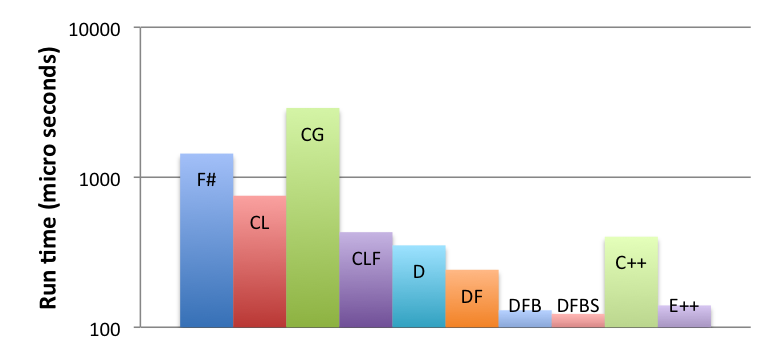
\includegraphics[width=\columnwidth]{results/micro_add3_runtime.png}
\subcaption{Runtime performance comparison of different approaches on adding three vectors of 100 elements for one million times.}
\label{fig:runtime_add3}
\end{subfigure}
\hfill
\begin{subfigure}[b]{.58\textwidth}
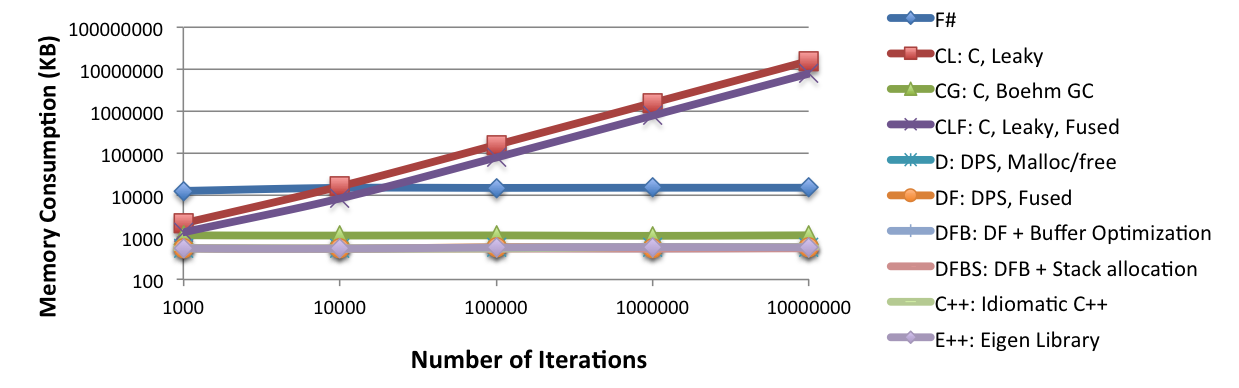
\includegraphics[width=\columnwidth]{results/micro_add3_mem.png}
\subcaption{Memory consumption comparison of different approaches on adding three vectors of 100 elements by varying the number of iterations. All the invisible lines are hidden under the bottom line.}
\label{fig:mem_add3}
\end{subfigure}
\begin{subfigure}[b]{.38\textwidth}
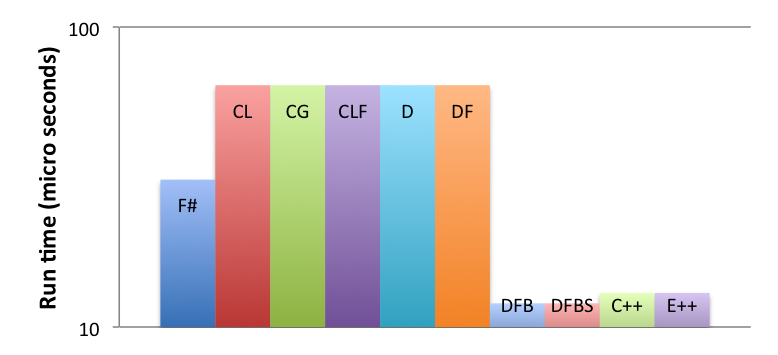
\includegraphics[width=\columnwidth]{results/micro_cross_runtime.png}
\subcaption{Runtime performance comparison of different approaches on cross product of two vectors of three elements for one million times.}
\label{fig:runtime_cross}
\end{subfigure}
\hfill
\begin{subfigure}[b]{.58\textwidth}
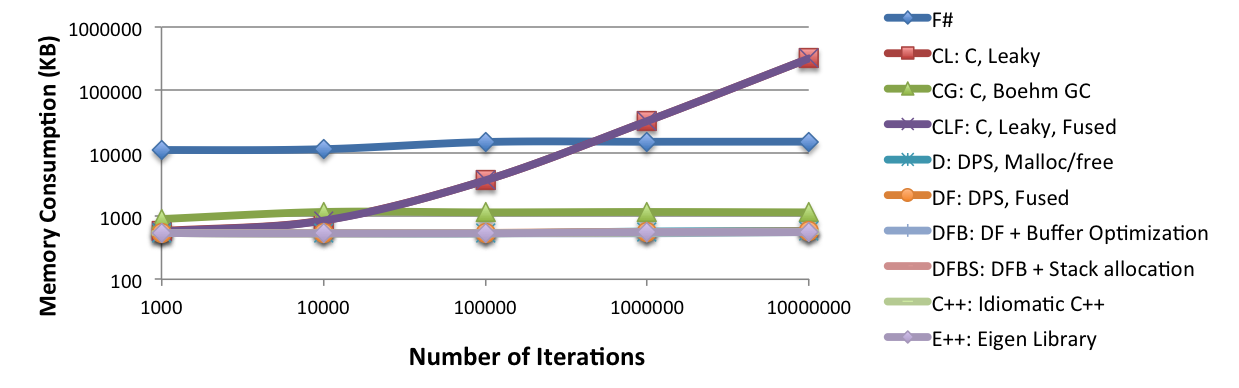
\includegraphics[width=\columnwidth]{results/micro_cross_mem.png}
\subcaption{Memory consumption comparison of different approaches on cross product of two vectors of three elements by varying the number of iterations.}
\label{fig:mem_cross}
\end{subfigure}
\caption{Experimental Results for Micro Benchmarks}
\label{fig:exp_micro}
\end{figure*}

Throughout this section, we compare the performance and memory consumption of the following alternatives:

%\def\apara#1{\noindent{\bf #1}}
\def\apara#1{\item {\bf #1}}
\begin{itemize}
\apara{F\#:} Using the array operations (e.g. map) provided in the standard library of F\# to implement vector operations.

\apara{CL: Leaky C code}, which is the generated C code from \lafsharp{}, using malloc to allocate vectors, never calling free.
\apara{CG: C code using Boehm GC}, which is the generated C code from \lafsharp{}, using \cod{GC\_malloc} of Boehm GC to allocate vectors.

\apara{CLF: CL + Fused Loops}, performs deforestation and loop fusion before CL.

\apara{D: DPS C code using system-provided malloc/free}, translates \lafsharp{} programs into \salafsharp{} before generating C code. Hence, the generated C code frees all allocated vectors. In this variant, the malloc and free functions are used for memory management.

\apara{DF: D + Fused Loops}, which is similar to the previous one, but performs deforestation before translating to \salafsharp{}. 
\apara{DFB: DF + Buffer Optimizations}, which performs the buffer optimizations described in Section~\ref{sec_simplification} 
(such as allocation hoisting and merging) on \salafsharp{} expressions. 

\apara{DFBS: DFB using stack allocator}, same as DFB, but using bump allocation for memory management, as previously discussed in Section~\ref{sec:ccodegen}.
This is the best C code we generate from \lafsharp{}.

\apara{C++: Idiomatic C++}, which uses an handwritten C++ vector library, depending on C++14 move construction and copy elision for performance, with explict programmer indication of fixed-size (known at compile time) vectors, permitting stack allocation.

\apara{E++: Eigen C++}, which uses the Eigen~\cite{guennebaud2010eigen} library which is implemented using C++ expression templates to effect loop fusion and copy elision. Also uses explicit sizing for fixed-size vectors.
\end{itemize}

First, we investigate the behavior of several variants of generated C code for two micro benchmarks. More specifically we see how DPS improves both performance and memory consumption in comparison with an F\# version. The behavior of the generated DPS code is very similar to manually handwritten C++ code and the Eigen library.

Then, we demonstrate the benefit of using DPS for some real-life computer vision and machine learning workloads motivated in~\cite{srajerbenchmark}. Based on the results for these workloads, we argue that using DPS is a great choice for generating C code for numerical workloads, such as computer vision algorithms, running on embedded devices with a limited amount of memory available. 
\subsection{Micro Benchmarks}

Figure~\ref{fig:exp_micro} shows the experimental results for micro benchmarks, one adding three vectors, the second using vector cross product.



\paragraph{add3}: vectorAdd(vectorAdd(vec1, vec2), vec3)\\ 
in which all the vectors contain 100 elements. This program is run one million times in a loop, and timing results are shown in Figure~\ref{fig:runtime_add3}.
In order to highlight the performance differences, the figure uses a logarithmic scale on its Y-axis. Based on these results we make the following observations.
First, we see that all C and C++ programs are outperforming the F\# program, except the one which uses the Boehm GC.
This shows the overhead of garbage collection in the F\# runtime environment and Boehm GC.
Second, loop fusion has a positive impact on performance. This is because this program involves creating an intermediate vector (the one resulting from addition of vec1 and vec2). 
Third, the generated DPS C code which uses buffer optimizations (DFB) is faster than the one without this optimization (DF). 
This is mainly because the result vector is allocated only once for DFB whereas it is allocated once per iteration in DF. Finally, there is no clear advantage for C++ versions.  This is mainly due to the fact that the vectors have sizes not known at compile time, hence the elements are not stack allocated. The Eigen version partially compensates this limitation by using vectorized operations, making the performance comparable to our best generated DPS C code.

The peak memory consumption of this program for different approaches is shown in Figure~\ref{fig:mem_add3}. This measurement is performed by running this program by varying number of iterations. Both axes use logarithmic scales to better demonstrate the memory consumption difference. As expected, F\# uses almost the same amount of memory over the time, due to garbage collection. However, the runtime system sets the initial amount to 15MB by default. Also unsurprisingly, leaky C uses memory linear in the number of iterations, albeit from a lower base.  The fused version of leaky C (CLF) decreases the consumed memory by a constant factor. Finally, DPS C, and C++ use a constant amount of space which is one order of magnitude less than the one used by the F\# program, and half the amount used by the generated C code using Boehm GC.


\begin{figure*}[t]
\begin{subfigure}[t]{.38\textwidth}
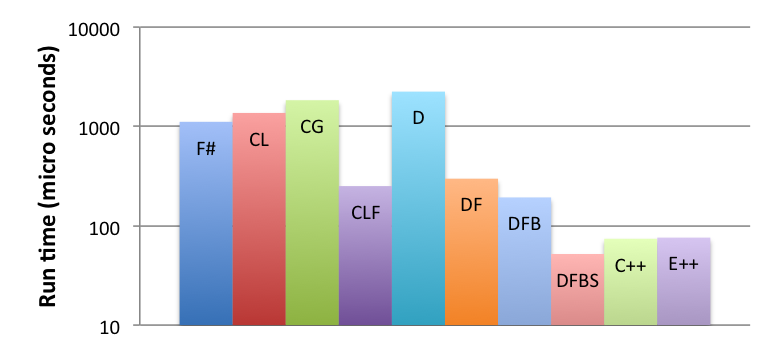
\includegraphics[width=\columnwidth]{results/proj_runtime.png}
\subcaption{Runtimes: Bundle Adjustment}
\label{fig:runtime_ba}
\end{subfigure}
\hfill
\begin{subfigure}[t]{.58\textwidth}
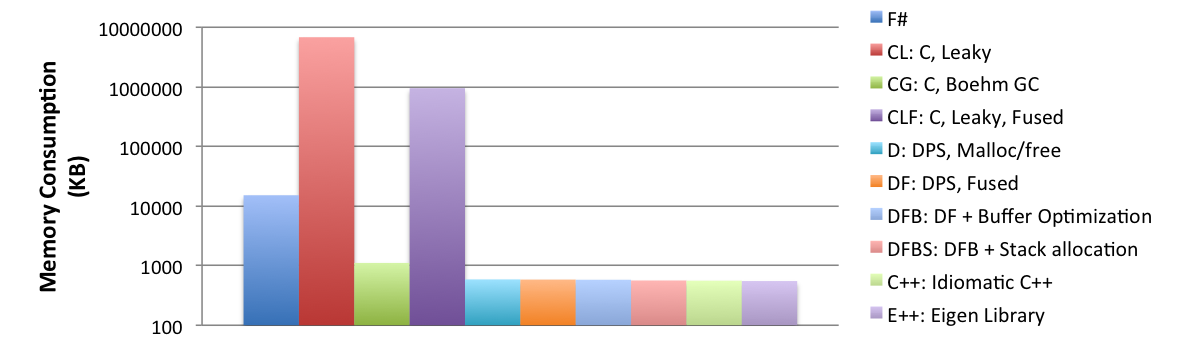
\includegraphics[width=\columnwidth]{results/proj_mem.png}
\subcaption{Memory consumption: Bundle Adjustment}
\label{fig:mem_ba}
\end{subfigure}
\begin{subfigure}[t]{.38\textwidth}
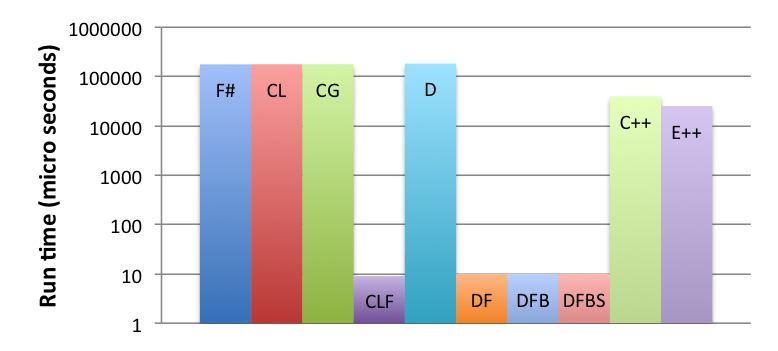
\includegraphics[width=\columnwidth]{results/gmm_runtime.png}
\subcaption{Runtimes: GMM}
\label{fig:runtime_gmm}
\end{subfigure}
\hfill
\begin{subfigure}[t]{.58\textwidth}
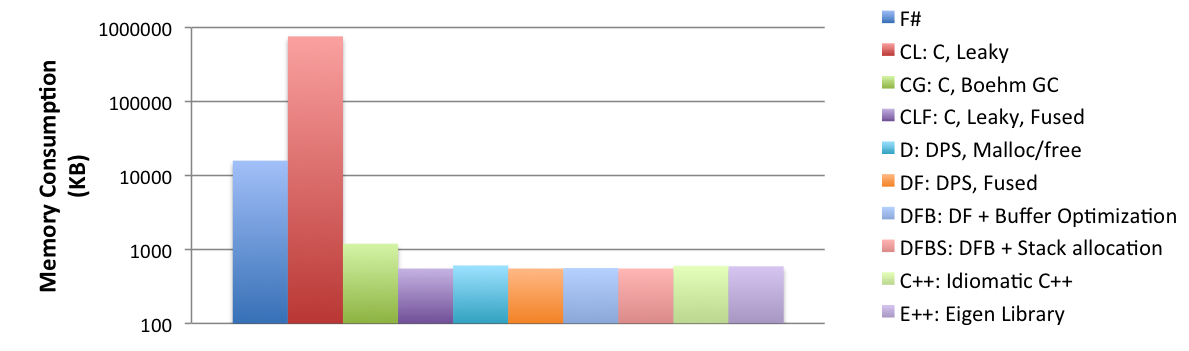
\includegraphics[width=\columnwidth]{results/gmm_mem.png}
\subcaption{Memory consumption: GMM}
\label{fig:mem_gmm}
\end{subfigure}
\begin{subfigure}[t]{.38\textwidth}
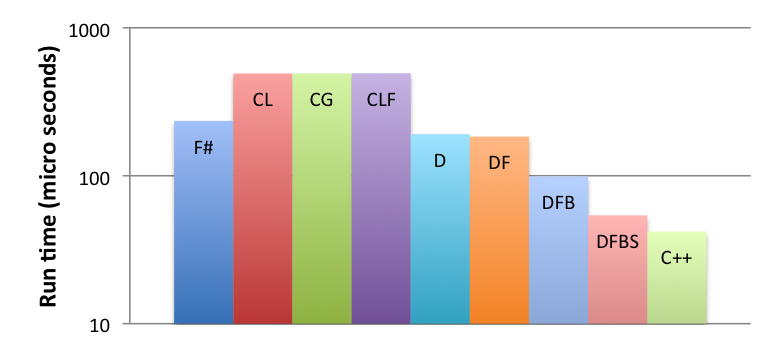
\includegraphics[width=\columnwidth]{results/ht_runtime.png}
\subcaption{Runtimes: Hand Tracking}
\label{fig:runtime_ht}
\end{subfigure}
\hfill
\begin{subfigure}[t]{.58\textwidth}
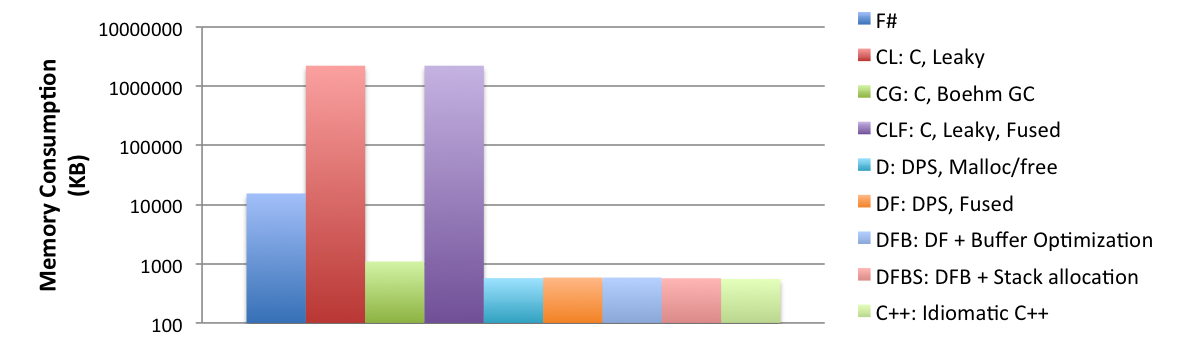
\includegraphics[width=\columnwidth]{results/ht_mem.png}
\subcaption{Memory consumption: Hand Tracking}
\label{fig:mem_ht}
\end{subfigure}
\caption{Experimental Results for Computer Vision and Machine Learning Workloads}
\end{figure*}

\paragraph{cross}: vectorCross(vec1, vec2)\\
This micro-benchmark is 1 million runs in which the two vectors contain 3 elements.  Timing results are in Figure~\ref{fig:runtime_cross}. 
We see that the F\# program is faster than the generated leaky C code, perhaps because garbage collection is invoked less frequently than in \emph{add3}. Overall, in both cases, the performance of F\# program and generated leaky C code is very similar.
In this example, loop fusion does not have any impact on performance, as the program contains only one operator. 
As in the previous benchmark, all variants of generated DPS C code have a similar performance and outperform the generated leaky C code and the one using Boehm GC, for the same reasons.
Finally, both handwritten and Eigen C++ programs have a similar performance to our generated C programs. For the case of this program, both C++ libraries provide fixed-sized vectors, which results in stack allocating the elements of the two vectors. This has a positive impact on performance. Furthermore, as there is no SIMD version of the cross operator, we do not observe a visible advantage for Eigen.

Finally, we discuss the memory consumption experiments of the second program, which is shown in Figure~\ref{fig:mem_cross}. This experiment leads to the same observation as the one for the first program. However, as the second program does not involve creating any intermediate vector, loop fusion does not improve the peak memory consumption.

The presented micro benchmarks show that our DPS generated C code improves both performance and memory consumption by an order of magnitude in comparison with an equivalent F\# program. 
Also, the generated DPS C code promptly deallocates memory which makes the peak memory consumption constant over the time, as opposed to a linear increase of memory consumption of the generated leaky C code. In addition, by using bump allocators the generated DPS C code can improve performance as well. 
Finally, we see that the generated DPS C code behaves very similarly to both handwritten and Eigen C++ programs.

Next, we investigate the performance and memory consumption of real-life workloads.

\subsection{Computer Vision and Machine Learning Workloads}
\paragraph{Bundle Adjustment} \cite{triggs1999bundle} is a  computer vision problem which has many applications. In this problem, the goal is to optimize several parameters in order to have an accurate estimate of the projection of a 3D point by a camera. This is achieved by minimizing an objective function representing the reprojection error.  This objective function is passed to a nonlinear minimizer as a function handle, and is typically called many times during the minimization.

One of the core parts of this objective function is the \emph{project} function which is responsible for finding the projected coordinates of a 3D point by a camera, including a model of the radial distortion of the lens. The \lafsharp{} implementation of this method is given in Figure~\ref{fig:ba_code}.
\begin{figure}[t]
\hfill\begin{minipage}{.75\textwidth}\raggedright
\lett{} radialDistort = \vabs{(radical: Vector) (proj: Vector)}{}\\
\tabt \lett{} rsq = vectorNorm proj\\
\tabt \lett{} L = 1.0 + radical.[0] * rsq + radical.[1] * rsq * rsq\\
\tabt vectorSMul proj L\\
\lett{} rodriguesRotate = \vabs{(rotation: Vector) (x: Vector)}{}\\
\tabt \lett{} sqtheta = vectorNorm rotation\\
\tabt \cod{if} sqtheta != 0. \cod{then}\\
\tabt\tabt \lett{} theta = sqrt sqtheta\\
\tabt\tabt \lett{} thetaInv = 1.0 / theta\\
\tabt\tabt \lett{} w = vectorSMul rotation thetaInv\\
\tabt\tabt \lett{} wCrossX = vectorCross w x\\
\tabt\tabt \lett{} tmp = (vectorDot w x) * (1.0 - (cos theta))\\
\tabt\tabt \lett{} v1 = vectorSMul x (cos theta)\\
\tabt\tabt \lett{} v2 = vectorSMul wCrossX (sin theta) \\
\tabt\tabt vectorAdd (vectorAdd v1 v2) (vectorSMul w tmp)\\
\tabt \cod{else} \\
\tabt\tabt vectorAdd x (vectorCross rotation x)\\
\lett{} project = \vabs{(cam: Vector) (x: Vector)}{}\\
\tabt\lett{} rotation = vectorSlice cam 0 2 \\
\tabt\lett{} center = vectorSlice cam 3 5 \\
\tabt\lett{} radical = vectorSlice cam 9 10 \\
\tabt\lett{} Xcam =  \\
\tabt\tabt rodriguesRotate rotation (vectorSub x center) \\
\tabt\lett{} distorted =  \\
\tabt\tabt radialDistort radical ( \\
\tabt\tabt \tabt vectorSMul ( \\
\tabt\tabt \tabt \tabt vectorSlice Xcam 0 1 \\
\tabt\tabt \tabt ) (1.0/Xcam.[2])) \\
\tabt vectorAdd (vectorSlice cam 7 8) ( \\
\tabt\tabt vectorSMul distorted cam.[6] \\
\tabt  )
\end{minipage}\hfill
\caption{Bundle Adjustment functions in \lafsharp{}.}
\label{fig:ba_code}
\end{figure}

Figure~\ref{fig:runtime_ba} shows the runtime of different approaches after running \emph{project} ten million times. First, the F\# program performs similarly to the leaky generated C code and the C code using Boehm GC. Second, loop fusion improves speed fivefold. Third, the generated DPS C code is slower than the generated leaky C code, mainly due to costs associated with intermediate deallocations. However, this overhead is reduced by using bump allocation and performing loop fusion and buffer optimizations. Finally, we observe that the best version of our generated DPS C code marginally  outperforms both C++ versions.

The peak memory consumption of different approaches for Bundle Adjustment is shown in Figure~\ref{fig:mem_ba}. First, the F\# program uses three orders of magnitude less memory in comparison with the generated leaky C code, which remains linear in the number of calls. This improvement is four orders of magnitude in the case of the generated C code using
Boehm GC. Second, loop fusion improves the memory consumption of the leaky C code by an order of magnitude, due to removing several intermediate vectors. Finally, all generated DPS C variants as well as C++ versions consume the same amount of memory. The peak memory consumption of is an order of magnitude better than the F\# baseline. 

\paragraph{The Gaussian Mixture Model} is a workhorse machine learning tool, used for computer vision applications such as image background modelling and image denoising, as well as semi-supervised learning. 

In GMM, loop fusion can successfully remove all intermediate vectors. Hence, there is no difference between CL and CLF, or between DS and DSF, 
in terms of both performance and peak memory consumption as can be observed in Figure~\ref{fig:runtime_gmm} and Figure~\ref{fig:mem_gmm}. Both C++ libraries do not support the loop fusion needed for GMM. Hence, they behave three orders of magnitude worse than our fused and DPS generated C code.

Due to the cost for performing memory allocation (and deallocation for DPS) at each iteration, the F\# program, the leaky C code, and the generated DPS C code exhibit a worse performance than the fused and stack allocated versions. Furthermore, as the leaky C code does not deallocate the intermediate vectors, it monotonically increases the consumed memory.

\paragraph{Hand tracking} is a computer vision/computer graphics workload~\cite{taylor2014user} that includes matrix-matrix multiplies, and numerous combinations of fixed- and variable-sized vectors and matrices.
Figure~\ref{fig:runtime_ht} shows performance results of running one of the main functions of hand-tracking for 1 million times. As in the \emph{cross} micro-benchmark we see no advantage for loop fusion, because in this function the intermediate vectors have multiple consumers. Similar to previous cases generating DPS C code improves runtime performance, which is improved even more by using bump allocation and performing loop fusion and buffer optimizations. However, in this case the idiomatic C++ version outperforms the generated DPS C code. Figure~\ref{fig:mem_ht} shows that DPS generated programs consume an order of magnitude less memory than the F\# baseline, equal to the C++ versions.

